\clearpage
\section{Direct SPI-state / SYS-reset correlation: 14 November 2026}
Four direct reset traces were captured with temporary image \texttt{56069fb9}.
At every SYS reset: \textbf{HSEL 0, HSCK 0, bit counter 0, reading 0}: decoded
parser IDLE, with the sampled debug-stability flag set. The parser has no
SYS reset input and had already been idle for 9.608--10.219 nominal ms after
frame completion. Thus the idle state is not produced by SYS resetting it.
The fixed SYS MMCM loses LOCK for 8.483--8.633 nominal us. Its RST/PWRDWN
remain zero; CAP and GTX PLL LOCK stay high in all four recorded windows.
\begin{center}\begin{tabular}{rrrr}\toprule
Divider & Read & Repeat & Delay after frame [ms]\\\midrule
601&0&0&10.219\\
601&1&0&9.608\\
601&0&1&9.632\\
601&1&1&10.060\\\bottomrule\end{tabular}\end{center}
All 12 saved frames have 64 sampled SCK transitions and correct signatures.
Divider 600 gives 0/6 reset captures ; 601 gives 4/6. Both read 2 repetitions at 601
are stable. This small ordered comparison suggests timing sensitivity but
does not establish phase, returned data or an electrical component as the cause.

\subsection{Actual netlist connections}
Original \texttt{c7531465} and observer routed checkpoints were audited.
SYS MMCM CLKIN1 is driven by IBUFDS\_GTE2/ODIV2 through BUFG; CLKINSEL is 1.
RST, PWRDWN, dynamic-phase and DRP write controls are tied to ground in both.
Feedback is its own CLKFBOUT, with INTERNAL compensation. SYS reset is the
FDPE synchronizer with asynchronous preset from inverted MMCM LOCK.
SPI inputs do not drive this inspected reset/clock-control cone. Targeted
MDRV/NSTD/UCIO checks find no violations. Shared constant-zero aliases to RAM
address bits are expected constants, not merged state signals.
SPI and clock package pins are distinct: HSCK G22, HSEL G26, HMOSI F25,
HMISO F24, MGTCLK H6/H5 and MCLK1 AA3/AA2.

\subsection{Coverage and limits}
Thirteen complete captures are retained: one idle and 12 stimulated. The
planned 56-window sweep stopped on an ancillary uptime-read timeout in the
first 602/read0 case. Its frozen records were read but not persisted before
the exception; that case is unknown and 42later windows were not attempted.
The save order is fixed for subsequent runs; original executed code is retained.
Four complete reset traces and their independently decoded states are valid.

Watch uses nominal 40.0787 MHz MCLK1 and survives SYS reset. SPI debug is sampled
multibit, not an atomic CDC transfer. Ignore first 8 ARM-settling ticks.
Timing is nominal running-clock time; a common watch/reference stop is not
represented. Ref-age maximum 102 ticks is not a phase-noise/glitch exclusion.
MISO is internal data, not physical voltage while tristated. No unique root
cause or active-parser-state correlation is established.

Exact \texttt{c7531465} was restored. Kasli was not reloaded; SPI stayed driven.
Power, frontend 0xfff and fresh physical ADC bankA on all 12 channels passed.
No explicit external PLL, MCU, CPLD, flash or analog changes. Candidate
WNS 0.066 ns/WHS 0.051 ns; simulation and DRC passed. Raw records, source/bit,
audit scripts/results and analysis are in \texttt{system/evidence-spi-state-20261114}.
\clearpage
\begin{figure}[p]\centering
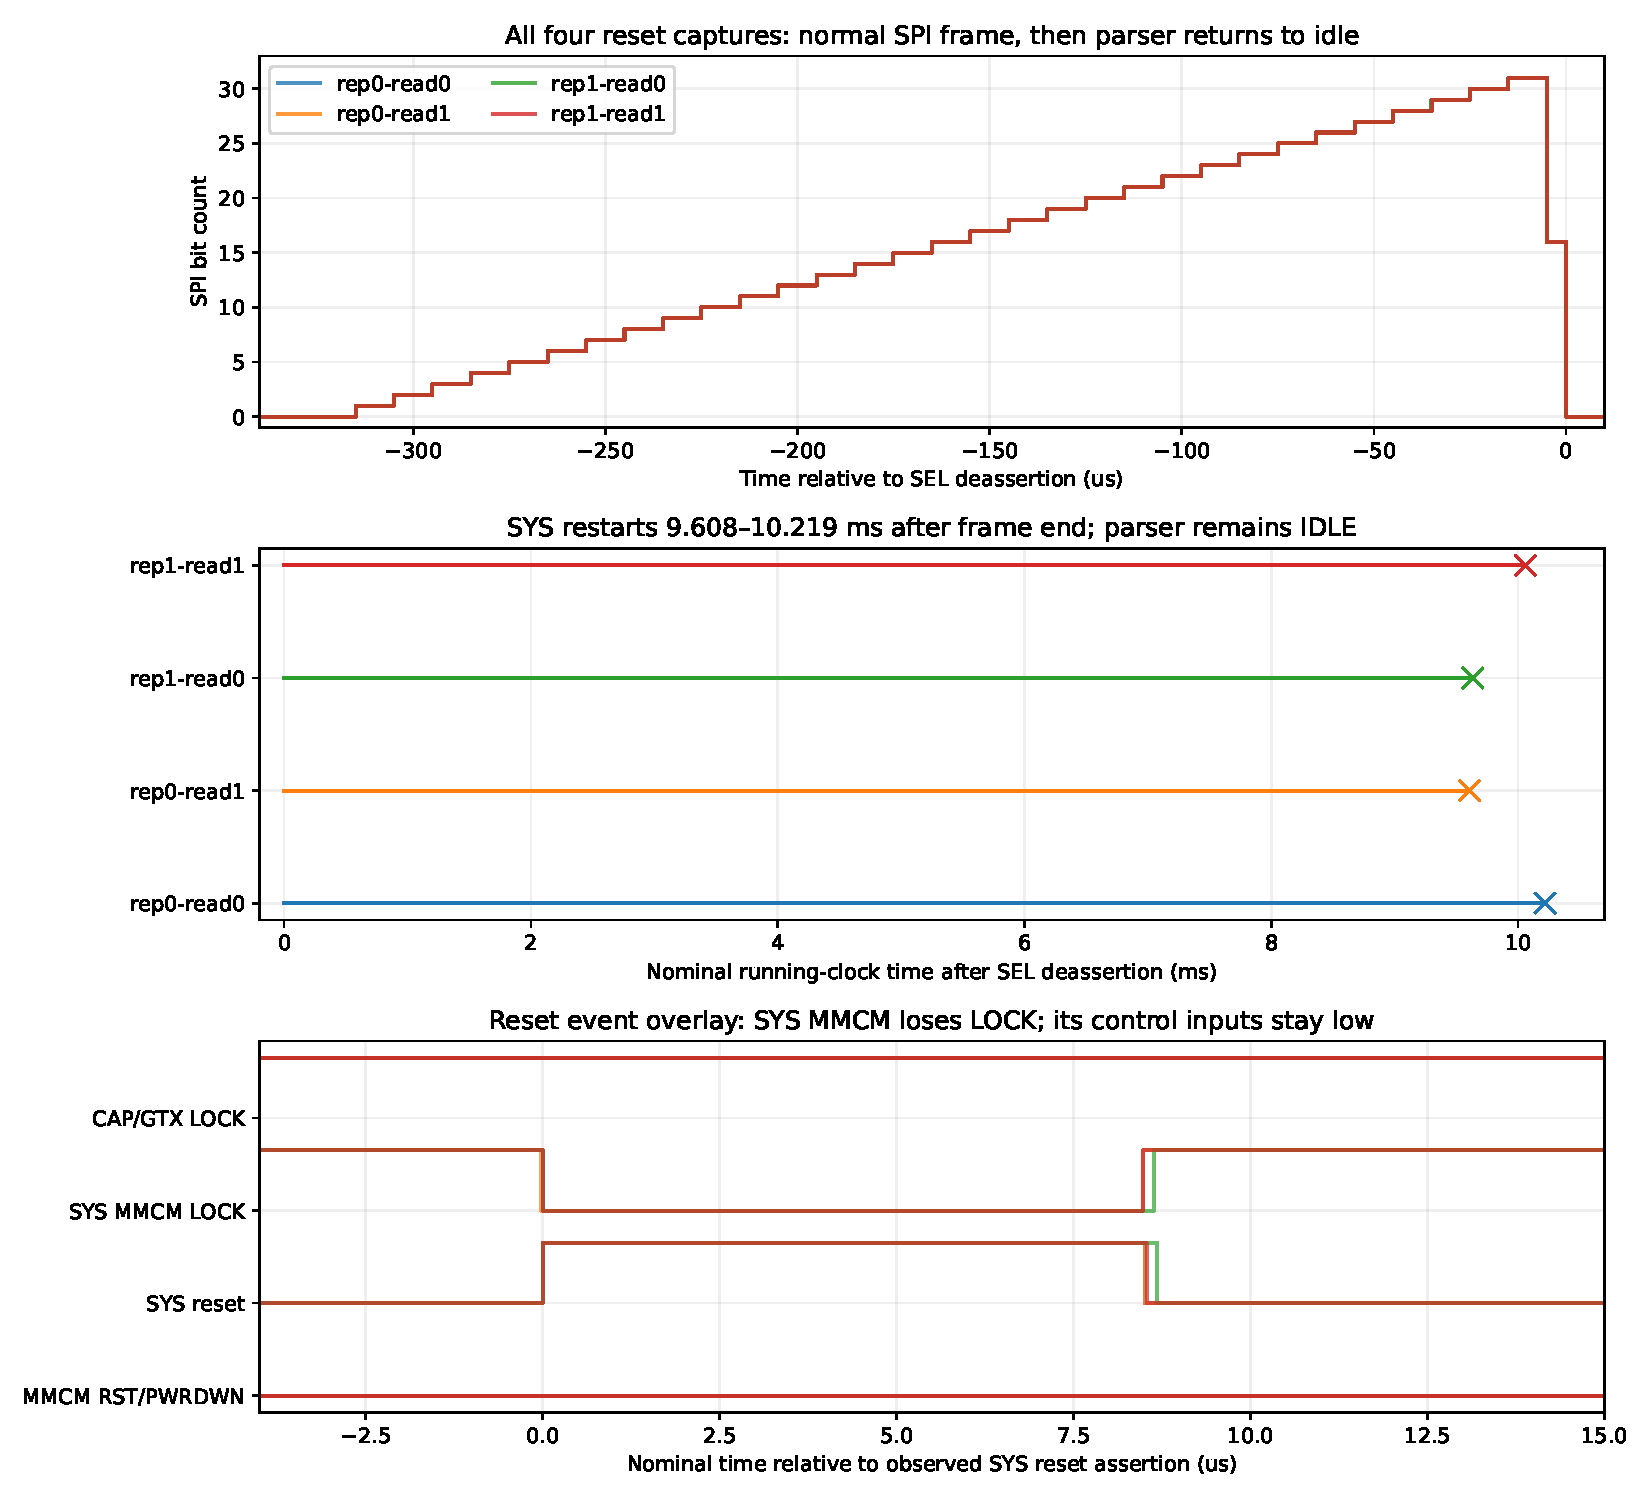
\includegraphics[width=\textwidth,height=.90\textheight,keepaspectratio]{spi-reset-state.pdf}
\caption{Four direct reset captures. Nominal sampled timing; the last state is
extended only within the programmed post-reset capture tail.}
\end{figure}\clearpage
